\section{Absorbing layer: energy conservation and Beer--Lambert limit}

With absorption present in a finite layer, the reflectance and the
transmittance no longer sum to unity; the missing fraction is deposited in
the film itself. This example verifies, first, that the TMM partitions the
incident power correctly ($R + T + A = 1$) and, second, that the
transmittance approaches the expected Beer--Lambert exponential for
optically thick films. The stack is an amorphous-silicon-like film
($n_f = 4.0 + 0.5\,\ii$) on glass ($n_s = 1.52$) in air ($n_0 = 1.00$) at
$\lambda = \SI{550}{\nano\metre}$.

Panel (a) sweeps the film thickness from $0$ to \SI{400}{\nano\metre} in
801 points. The TMM returns the reflectance $R$, the transmittance $T$ and
the per-layer absorption $A$ (here a single scalar because there is only
one finite layer). The three components oscillate through Airy fringes as
$d$ grows, but energy conservation
\begin{equation}
  R + T + A = 1 \label{eq:abs-rta}
\end{equation}
must hold at every point. Panel (b) extends the scan out to
\SI{2000}{\nano\metre}, where the Airy ripple in $T(d)$ decays into the
Beer--Lambert asymptote
\begin{equation}
  T(d) \longrightarrow T_{\rm if}\,e^{-\alpha d},\qquad \alpha = \frac{4\pi\,\Imy(n_f)}{\lambda}, \label{eq:abs-BL}
\end{equation}
with the interface transmittance
$T_{\rm if} = (1 - R_{\rm front})(1 - R_{\rm back})$ built from the two
single-interface reflectances. At $\lambda = \SI{550}{\nano\metre}$ the
numerical values are $\alpha \approx \SI{1.14e-2}{\per\nano\metre}$, i.e.\
a penetration depth $1/\alpha \approx \SI{87.5}{\nano\metre}$.

\begin{center}
\begin{tikzpicture}
  \fill[black!4] (0, 0) rectangle (5, 1.6);
  \fill[orange!20] (0,-0.7) rectangle (5, 0);
  \fill[blue!6]  (0,-1.9) rectangle (5,-0.7);
  \draw[thick] (0,0) -- (5,0);
  \draw[thick] (0,-0.7) -- (5,-0.7);
  \node[lbl, anchor=east] at (4.9, 1.2) {air};
  \node[lbl, anchor=east] at (4.9,-0.35) {a-Si, $d$};
  \node[lbl, anchor=east] at (4.9,-1.4) {glass};
  \raysketch{1.6}{0}{t}
\end{tikzpicture}
\end{center}

\begin{figure}[!htbp]
  \centering
  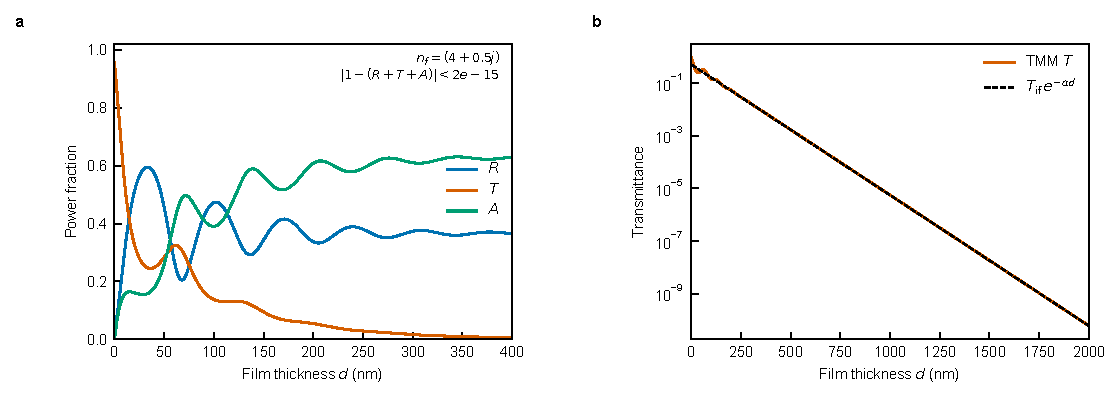
\includegraphics[width=\textwidth]{07_absorbing_layer.pdf}
  \caption{(a) Reflectance $R$, transmittance $T$ and per-layer absorption $A$ as a function of film thickness. (b) $T(d)$ on a logarithmic scale out to \SI{2000}{\nano\metre}, with the Beer--Lambert envelope $T_{\rm if}\,e^{-\alpha d}$ as a reference.}
  \label{fig:absorb}
\end{figure}

Equation~\eqref{eq:abs-rta} is satisfied to
$\max|1 - (R + T + A)| \approx \num{2e-15}$ over the whole thickness
scan, which confirms the per-layer absorption formula derived from the
Poynting flux balance. For $d \gtrsim 1/\alpha$ the oscillatory Fabry--Pérot
modulation of $T(d)$ dies out, and beyond a few absorption lengths the TMM
curve locks onto the exponential envelope of~\eqref{eq:abs-BL} without
adjustable parameters. The transition from coherent interference to the
Beer--Lambert regime is therefore reproduced smoothly by the same
formalism.


